\subsection{Analiza architektur zamkniętych pętli sterowania ENI}\hypertarget{sec:25}{}

\subsubsection{Typy pętli sterowania}

Większość architektur pętli sterowania dla systemów kognitywnych i adaptywnych używa mechanizmów:
\begin{itemize}
    \item sprzężenia zwrotnego (ang. \textit{ang. feedback}) - mechanizm, w którym system reaguje na swoje wyjście i dostowosuje swoje działanie na podstawie wyników,
    \item sprzężenia wyprzedzającego (ang. \textit{ang. feedforward}) - mechanizm, w którym system przewiduje przyszłe zmiany i podejmuje działania, zanim błąd faktycznie się pojawi.
\end{itemize}

Te sygnały odgrywają kluczową rolę w stabilizowaniu systemu, ale też jego umiejętności empirycznego uczenia się. Pętlę, która wykorzystuje mechanizm feedbacku nazywamy \textbf{zamkniętą}.

\textbf{Hierarchiczna} koordynacja (organizacja) pętli przypomina drzewo. Organizacja ta pozwala, aby różne decyzje podejmowane były przez rożne węzły drzewa. W ogólności, istnieje zestaw nadrzędnych (ang. \textit{supervisory}) pętli, które alokują zadania do pętli podwładnych (ang. \textit{subordinary}). Każda podrzędna pętla wykonuje swoje zadania i zwraca rezultaty do swojej pętli nadrzędnej. 

Zaawansowane zastosowania pozwalają jednej grupie dedykowanych pętli przejąć kontrolę nad hierarchią w zależności od celów i zmian w środowisku. 


\begin{figure}[!h]
    \centering 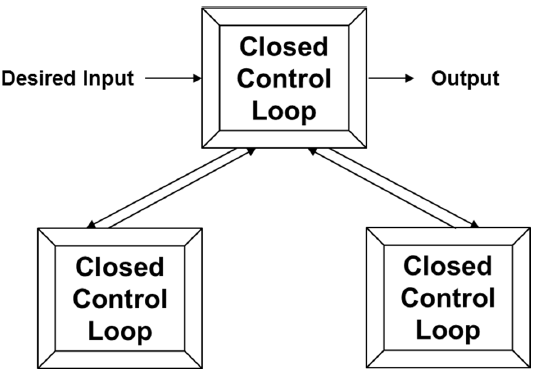
\includegraphics[width=1\linewidth]{25-hierachical.png}
    \caption{Hierarchiczna organizacja zamkniętych pętli sterowania}\label{fig:25-hierachical}
\end{figure}

Pętla \textbf{rozproszona} składa się z komponentów działających w różnych lokalizacjach, które komunikują się ze sobą poprzez mechanizmy przesyłania wiadomości. 

\textbf{Adaptacyjność} pętli to dostosowywanie jej parametrów sterowania w czasie rzeczywistym albo na podstawie modelu, który definiuje pożądany efekt, albo używając analizy statystycznej do budowania modelu na podstawie mierzonych danych.

\textbf{Federacją} nazywamy grupę pół autonomicznych pętli sterowania, które używają formalnych kontraktów, aby regulować ich wzajemną interakcję i zachowania. Kontrakty obejmują zasady przyjmowania nowych członków federacji, regulacje dotyczące widoczności i rodzaju informacji jakie mogę być udostępnianie innym członkom federacji. Każda pętla federacji operuje na swoich lokalnych danych. Następnie decyzje podjęte przez każdą z nich są agregowane i publikowane. 

\textbf{Kognitywną} pętla sterowania nazywamy taką, która z pośród dostępnych jej danych jest w stanie wyrozumować nowe dane, informację i finalnie wiedzę, która pomoże jej osiągać cele zarządzania.